\chapterauthor{Tim Warburton}

\epigraph{Didn’t I tell you? I’ve got a brain the size of the planet. No one ever listens to me of course.}{Marvin the Paranoid Android, \emph{The Hitch-Hiker's Guide to the Galaxy}.}

\minitoc

%% MPI Part I
%%
%% Introduction 
%%   Limits on shared memory systems
%%

%% MPI notation

\section{Why MPI?}

Our initial foray into parallel computing with OpenMP was relatively simple just requiring a few API calls and compiler directives to distribute work amongst CPU cores. Unfortunately, attractive as that approach is it is ultimately limited to the maximum number of CPU cores and system memory available on a given shared memory system. Nowadays it is possible to build a shared memory system with more than 50 cores and say a few terabytes (trillion byte) of shared memory. However, what if we need more than a few terabytes and a lot more CPU cores to reduce compute time ? That is currently pretty much the end of the road for programming CPUs with OpenMP.

The \href{https://en.wikipedia.org/wiki/Message_Passing_Interface}{Message Passing Interface (MPI)} emerged in the 1990s as a standard for distributed computing. The standard defines a set of functions for a comprehensive set of communication operations. The goal of MPI is to enable multiple instances of a program to collaborate on a task even though they might be executing on networked computers distributed around the world.  We will refer to each instance among the set of running MPI programs as an MPI process or sometimes MPI rank. Allowing MPI processes to execute on multiple systems sidesteps the shared memory restriction inherent in the OpenMP standard.

Point-to-point communications patterns are specified so that data can be sent between MPI processes. Collective communication patterns are specified so that groups of MPI processes  can perform round-robin data exchanges, sum distributed data variables, broadcast data from one MPI process to all other processes. Each of these operations can be performed by a call to an MPI API function.

The \href{https://www.mpi-forum.org/docs/}{MPI standard} has evolved over time and now standards at version 3.1. Since the first version was ratified new capabilities have been added to the standard. Experience using MPI for distributed computing has revealed gaps in prior standards and some proposals for new capabilities have been accepted by the standards committee and added to updated versions of the MPI standard.

The MPI standard is distinct from the actual implementations, although sometimes the software packages that provide the MPI advanced programming interface are themselves (somewhat mistakenly) referred to as MPI. Notable examples of actual distributed computing libraries that support the MPI API include: \href{https://www.open-mpi.org}{open-mpi}, \href{https://www.mpich.org}{MPICH}, \href{http://mvapich.cse.ohio-state.edu}{MVAPICH}, \href{http://software.intel.com/mpi}{Intel MPI}, and \href{https://docs.microsoft.com/en-us/message-passing-interface/microsoft-mpi}{Microsoft MPI}. Initially in this class we will use  \href{https://www.mpich.org}{MPICH} developed in part by researchers at Argonne National Lab as it is easily installed in your VirtualBox as described later in this lecture.

The bottom line is that if the problem you want to attack is too large for any single computer then distributing the problem amongst multiple computers with MPI providing communication links between them is a solid approach. The downside is that now you need to write programs that will not be executed by one computer but possibly many computers and you are responsible for implementing any message passing between the computers through MPI API calls.

See \href{https://en.wikipedia.org/wiki/Parallel_computing}{wiki} for an overview of parallel computing including a discussion on \href{https://en.wikipedia.org/wiki/Flynn%27s_taxonomy}{Flynn's Taxonomy}.

\section{MPI: hello world}

In this section we follow the time honored tradition of starting MPI with a hello world program to start familiarization with the MPI API. This is the same approach that we used for C, Python, and OpenMP. This hello world example is very similar to \texttt{ompHelloWorld.c} but the specifics are rather different.

The following program is compiled with the \texttt{mpicc} compiler and has to be run with the \texttt{mpiexec} (or \texttt{mpirun}) MPI launcher. Both of these command apps ship with most MPI development packages. Without further ado here is the MPI hello world:

\begin{minted}{c}
/* L16/mpiHelloWorld.c */

#include <mpi.h>
#include <stdio.h>

int main(int argc, char **argv){

 /* initialize MPI library communication system */
 MPI_Init(&argc, &argv);
 
 /* each rank prints hello world message */
 printf("MPI Hello World !\n");
 
 /* all ranks must shut down MPI library comms */
 MPI_Finalize();
 
 /* return as usual */
 return 0;
}
\end{minted}

Some notes:

{\bf Note \#1}: we must include the \texttt{mpi.h} header file. It includes function prototypes for more than 500 MPI functions collected in the MPI API and library implementation.

{\bf Note \#2}: when we want to run an MPI program we launch it using the \texttt{mpiexec} MPI launcher. At that point we specify (amongst other things) how many instances of the program we want to launch. If we say that we want to run 10 instances of the program then \texttt{mpiexec} will execute the program 10 times as a background task. Each of the 10 instances will be referred to henceforth as an MPI process (or process for short) or sometimes MPI rank (or rank for short).

{\bf Note \#3}: the MPI best practice guides suggest calling the MPI initialization function (\texttt{MPI\_Init} as soon as possible after the start of the \texttt{main} function. \texttt{MPI\_Init} is responsible for setting up communications between all ranks.

{\bf Note \#4}: to properly terminate an MPI program each process should call \texttt{MPI\_Finalize} prior to exiting. This guarantees that no rank will mysteriously hang while waiting to communicate with a process that has already exited.

{\bf Note \#5}: all MPI processes have independent memory spaces and independent call stacks. There is no memory sharing between MPI processes and this makes it very different to the shared memory model of OpenMP.

\section{Installing MPI and then compiling and running MPI code}

In the following we show how to install the MPICH implementation of MPI (you only need to do this once), then  how to compile the \texttt{mpiHelloWorld.c} program using the MPI C compiler \texttt{mpicc}, and finally to run the \texttt{mpiHelloWorld} program with 4 processes using \texttt{mpiexec}.

\myvbox[mytermbg]{\# install MPICH ( you only need to install MPICH once )\\ sudo apt-get install mpich \\ \\ \# build mpiHelloWorld using mpicc \\ mpicc -o mpiHelloWorld mpiHelloWorld.c \\ \\ \# run mpiHelloWorld with 4 processes \\ mpiexec -n 4 ./mpiHelloWorld }

When I run this in my VirtualBox I get some interesting output 
\begin{Verbatim}[frame=single]
mpiexec -n  4 ./mpiHelloWorld
MPI Hello World !
MPI Hello World !MPI Hello World !MPI Hello World !



\end{Verbatim}

Notice that extra white space is a biproduct of the way that the MPI processes operate independently. They have stepped on each other when writing to \texttt{stdout}. Their messages are merged together and on the second line three hello world messages have preempted each other's next-line control characters.

\boximagelabel{figures/L16/CMDA3634FA19MPITimelineHelloWorld-crop.pdf}{Cartoon timeline for the MPI hello world example: \texttt{mpiHelloWorld.c}}{MPItimelineCartoon.fig}

If you don't quite understand the timeline, please consider the cartoon in Figure \ref{MPItimelineCartoon.fig}. When the \texttt{mpiexec} command launches the MPI processes (shown as red/orange/green/purple lines), they each start at slightly different times and then each call \texttt{MPI\_Init} at slightly different times, they each print at different times, and they each enter  \texttt{MPI\_Finalize} independently and finally they all terminate only after all processes enter  \texttt{MPI\_Finalize}. This lack of synchronization between processes is a hallmark of MPI computations. Each process is really just an independently executing instance of the program. The processes only synchronize if they actually request to through the MPI API.

\section{MPI: note on notation}

As you are already beginning to see there is a somewhat uniform naming convention for MPI. 

\subsection{MPI: function names}
A typical function has the name: 

\texttt{MPI\_[Operation]}

Where the first letter of the operation name is capitalized. A typical example is the MPI function to send a message:

\texttt{MPI\_Send}

For an operation name with multiple words then the second and further words in the name are lower case, as in the function that reports the number of MPI processes: 

\texttt{MPI\_Comm\_rank}

\subsection{MPI: defines}

MPI defines are capitalized. There are MPI several defined quantities, for example to denote the types of entries in a message we use \texttt{MPI\_[TYPE]}.  Examples of variable types:

\texttt{MPI\_INT}, \texttt{MPI\_FLOAT}, \texttt{MPI\_DOUBLE}, \texttt{MPI\_CHAR}.


\section{MPI: rank and size}

The \texttt{mpiHelloWorld.c} example is straight forward albeit rather limited. After the MPI processes and initialize they do their own thing until they come together to finalize. This could have been achieved by writing a script to run the same program 4 times. However, things get more interesting when an MPI process queries the MPI API to find out how many processes were launched (``\texttt{size}'' in MPI terminology) and to  obtain a unique integer in the range \texttt{[0,size)}. For instance with this information a programmer can implement a different set of instructions for each MPI process. 

We now revisit the example from OpenMP where we output thread number information from each thread in a parallel region. In the MPI version that follows we use the \texttt{MPI\_Comm\_rank} and \texttt{MPI\_Comm\_size} API calls to obtain the MPI process rank and the number of MPI processes respectively.

\begin{minted}{c}
/* L16/mpiRankSize.c */

#include <mpi.h>
#include <stdio.h>

int main(int argc, char **argv){

 /* initialize MPI library communication system */
 MPI_Init(&argc, &argv);
 
 /* find rank index of current process */
 int rank;
 MPI_Comm_rank(MPI_COMM_WORLD, &rank);
 
 /* find number of current processes */
 int size;
 MPI_Comm_size(MPI_COMM_WORLD, &size);
 
 /* each rank prints hello world message with rank and size info*/
 printf("MPI Hello World from process %d of %d!\n", rank, size);
 
 /* all ranks must shut down MPI library comms */
 MPI_Finalize();
 
 /* return as usual */
 return 0;
}
\end{minted} 

{\bf Note \#1}: here \texttt{MPI\_COMM\_WORLD} is shorthand meaning for the processes in the global MPI communicator, i.e. all the MPI processes. 

{\bf Note \#2}: the \texttt{size} of the global MPI communicator is determined by how many processes \texttt{mpiexec} was instructed to set up with the \texttt{-n} command line argument. 

{\bf Note \#3}: \texttt{rank} is an integer number for the MPI process in the range \texttt{[0,size)}. 


The code output for a sample run is

\begin{Verbatim}[frame=single]
mpiexec -n 4 ./mpiRankSize
MPI Hello World from process 3 of 4!
MPI Hello World from process 2 of 4!
MPI Hello World from process 1 of 4!
MPI Hello World from process 0 of 4!
\end{Verbatim}
{\bf Note}: just like with OpenMP the MPI processes output their strings in no particular order. 

Repeating with 8 MPI processes we get

\begin{Verbatim}[frame=single]
mpiexec -n 8 ./mpiRankSize
MPI Hello World from process 6 of 8!
MPI Hello World from process 5 of 8!
MPI Hello World from process 7 of 8!
MPI Hello World from process 4 of 8!
MPI Hello World from process 2 of 8!
MPI Hello World from process 3 of 8!
MPI Hello World from process 1 of 8!
MPI Hello World from process 0 of 8!
\end{Verbatim}

Running again

\begin{Verbatim}[frame=single]
mpiexec -n 8 ./mpiRankSize
MPI Hello World from process 5 of 8!
MPI Hello World from process 2 of 8!
MPI Hello World from process 7 of 8!
MPI Hello World from process 4 of 8!
MPI Hello World from process 3 of 8!
MPI Hello World from process 0 of 8!
MPI Hello World from process 1 of 8!
MPI Hello World from process 6 of 8!
\end{Verbatim}

Later we will discuss how to nominate a single thread to output messages so that the output from the code will be the same every time it runs.

\section{MPI: thread divergence}

Now that we know how to distinguish between different MPI processes based on their MPI rank we can revisit the thread divergence example from OpenMP. In this example MPI processes with odd rank print a different message than MPI processes with even rank.

\begin{minted}{c}
/* L16/mpiThreadDivergence.c */

#include <mpi.h>
#include <stdio.h>

int main(int argc, char **argv){

 /* initialize MPI library communication system */
 MPI_Init(&argc, &argv);
 
 /* find rank index of current process */
 int rank;
 MPI_Comm_rank(MPI_COMM_WORLD, &rank);

 /* even ranks output hello */
 if((rank%2)==0)
   printf("MPI Hello World from even process %d!\n", rank);
 else /* odd ranks output goodbye */
   printf("MPI Goodbye World from odd process %d!\n", rank);
 
 /* all ranks must shut down MPI library comms */
 MPI_Finalize();
 
 /* return as usual */
 return 0;
}
\end{minted} 
In this code we used the modulo operator (\%) to obtain the remainder of the \texttt{rank} divided by 2 and print out a message chosen according to whether the remainder is zero or one. The output for an example 8 process run is 
\begin{Verbatim}[frame=single]
mpiexec -n 8 ./mpiThreadDivergence
MPI Goodbye World from odd process 3!
MPI Goodbye World from odd process 5!
MPI Goodbye World from odd process 1!
MPI Hello World from even process 6!
MPI Hello World from even process 2!
MPI Goodbye World from odd process 7!
MPI Hello World from even process 0!
MPI Hello World from even process 4!
\end{Verbatim}

So no surprises here, the code behaves as we expect. It is important however to recall here that each MPI process maintains its own totally independent memory space. Each process has its own call stack with process local stack variables and code counter. Each process also has its own heap memory space \footnote{There is a subtlety that since we are running an MPI program on a single VirtualBox that the data for all the processes does reside in the same physical space but that physical space is partitioned as far as the processes are concerned.}

\section{MPI: point to point messaging with two ranks}

This far the MPI processes have only interacted during the \texttt{MPI\_Init} and \texttt{MPI\_Finalize} operations when the MPI library sets up communication patterns between the MPI processes. In this section we introduce a point-to-point communication pattern where two MPI processes engage in an exchange of data. In particular one process sends data to a second process.

There are numerous ways to perform every  communication pattern you can imagine between two processes. In the following we use a ``blocking'' communication protocol where rank zero sends data to rank one using \texttt{MPI\_Send}, and rank one actively receives data from rank zero using \texttt{MPI\_Recv}. The blocking send in this context means that \texttt{MPI\_Send} does not return until data from the outgoing message buffer has been copied out of the buffer by MPI, i.e. the message is on its way to the destination. The blocking receive means that \texttt{MPI\_Recv} does not return until data from the incoming message has been copied into the incoming message buffer by MPI, i.e. the function does not return until the message has arrived.

\begin{minted}{c}
#include <mpi.h>
/* L16/mpiSendRecv.c */
/* two ranks, with rank 0 sending a message to rank 1 */
int main(int argc, char **argv){
 /* initialize MPI library comms  */
 MPI_Init(&argc, &argv);
 
 /* find rank index of current process */
 int rank;
 MPI_Comm_rank(MPI_COMM_WORLD, &rank);

 int N = 10; /* length of message to exchange */
 int n, tag = 999; /* message tag */
   
 if(rank==0){ /* rank 0 sends a message to rank 1 */
   int *outBuffer = (int*) calloc(N, sizeof(int));
   int dest = 1;
   
   for(n=0;n<N;++n) outBuffer[n] = n; 
   
   /* blocking send of data to rank 1 */
   MPI_Send(outBuffer, N, MPI_INT, dest, tag, MPI_COMM_WORLD);
 }
 
 if(rank==1){/* rank 1 receives message from rank 0 */
   MPI_Status status;
   int *inBuffer = (int*) calloc(N, sizeof(int));
   int source = 0;
   
   /* blocking receive of data from rank 0 */
   MPI_Recv(inBuffer, N, MPI_INT, source, tag, MPI_COMM_WORLD, &status);
   
   for(n=0;n<N;++n){ /* print received entries */
     printf("received: inBuffer[%d]=%d\n", n, inBuffer[n]);
   }
 }
 
 MPI_Finalize(); /* shut down MPI library comms */
 return 0;
}
\end{minted} 

The abstraction provided by the MPI API hides a large amount of machinery behind the scenes even in this relatively simple one way message exchange. To start with when the \texttt{MPI\_Send} is called by rank 0 it (potentially) starts a hand shaking process with rank 1 by sending a short message of intent to send a message. When rank 1 calls \texttt{MPI\_Recv} a response message will probably be sent that it is ready to receive the message. When rank 0 receives the handshake response it will start to send the data from the message buffer. Meanwhile every time messages are sent the data has to propagate through multiple levels of the \href{https://en.wikipedia.org/wiki/OSI_model}{Open Systems Interconnection (OSI)}. Of course all of this activity is hidden behind these innocuous looking \texttt{MPI\_Send} and \texttt{MPI\_Recv} calls and in a nutshell this simplified abstraction of complex network protocols is why MPI is the dominant communications library used in computational science. 

\boximagelabel{figures/L16/CMDA3634FA19MPITimelineSendRecv-crop.pdf}{Cartoon timeline for point-to-point communication using  \texttt{MPI\_Send} and \texttt{MPI\_Recv}.}{mpiSendRecv.fig}

The abstracted send/recv communication pattern is illustrated in Figure \ref{mpiSendRecv.fig}.

\section{MPI: serialization when all but one process send a message up to neighbor process}

In this section we consider the case when  process number \texttt{rank} sends a message to the process with \texttt{rank+1}. This is a common communication pattern in particular in numerical PDE simulation codes.

To illustrate what can go wrong with this simple communication pattern we present a  stripped down pseudo-code. This pseudoo-code is not complete and needs to be finished to actually compile.

\begin{minted}{c}
 /* PSEUDO-CODE: this code may serialize */
 if(rank<size-1){ /* send to rank+1 */
    MPI_Send data from outBuffer to rank+1;
 }

 if(rank>0) { /* receive from rank-1 */
    MPI_Recv data into inBuffer from rank-1
 }
\end{minted}

\begin{Exercise}
\label{mpiSmallMessageBlocked.ex}
Assume that the message size is small enough that MPI will immediately copy the data from the outgoing buffer into an internal MPI buffer so that  \texttt{MPI\_Recv} returns quickly.
\underline{Sketch the timeline for 6 ranks.}
\end{Exercise}

A cartoon sketch is given on the next page to illustrate a typical time line for this communication pattern for small  message sizes.

\newpage

\begin{Answer}
{\bf Timeline sketch for Exercise \ref{mpiSmallMessageBlocked.ex}}: if the message being sent to \texttt{rank+1} is small enough the send and receive happen relatively quickly. The cartoon timeline sketch
shows the only causal constraint that the \texttt{MPI\_Recv} on process \texttt{rank+1} cannot finish before the \texttt{MPI\_Sendd} on process \texttt{rank} starts, i.e. the data movement arrows must point forward in time since messages cannot travel backwards in time.
\end{Answer}

\boximagelabel{figures/L16/CMDA3634FA19MPITimelineSendUpSmall-crop.pdf}{Cartoon timeline when sending a \underline{small} message to \texttt{rank+1} using the blocking \texttt{MPI\_Send} and \texttt{MPI\_Recv}.}{mpiSendUpSmall.fig}


\begin{Exercise}
\label{mpiLargeMessageBlocked.ex}
Assume that the message size is large enough that MPI will not immediately copy the data from the outgoing buffer into an internal MPI buffer so that the receiving process has to post an \texttt{MPI\_Recv} before the \texttt{MPI\_Send} returns. \underline{Sketch the timeline for 6 ranks.}
\end{Exercise}

A cartoon sketch is given on the next page to illustrate a typical time line for this communication pattern for small  message sizes.

\newpage
\begin{Answer}
{\bf Timeline sketch for  for Exercise \ref{mpiLargeMessageBlocked.ex}}: if the message being sent to \texttt{rank+1} is large enough the send on process \texttt{rank} cannot finish until the receive starts on \texttt{rank+1}.  The cartoon timeline sketch
shows that to get started process with \texttt{rank=size-1} must receive the message from \texttt{rank=size-2} before that rank can start to receive the message from \texttt{rank=size-3} so we see a cascading waiting game with \texttt{rank=0} blocking inside the \texttt{MPI\_Send} until all the other processes have sent their messages. 
\end{Answer}

\boximagelabel{figures/L16/CMDA3634FA19MPITimelineSendUpLarge-crop.pdf}{Cartoon timeline when sending a \texttt{large} message to \texttt{rank+1} using the blocking \texttt{MPI\_Send} and \texttt{MPI\_Recv}.}{mpiSendUpSmall.fig}

In practice the internal MPI message buffer size will dictate which of these communication pattern actually happens for this type of chained message passing. 


The potential for unintended serialization demonstrated in Exercise \#2 where large data transfers caused a wait queue while the processes stalled in handshaking should be a wake up call. The MPI message passing abstraction is deceptively simple but can trip you up. Sketching what you think will happen in a communication pattern is a useful approach to avoid some issues.

In the next lecture we will start using the Message Passing Environment with MPI and the Jumpshot visualization tool to generate and explore timelines of actual MPI code executing. 

\section{MPI: possible deadlock with blocking point-to-point}

In the last section we saw how it is ``easy'' to create a serialization of point-to-point messaging in the case when each process tries to send a large message to process with rank+1 if that rank exists.

Now consider this piece of pseudo-code.

\begin{minted}{c}
 /* PSEUDO-CODE: this code may deadlock */
 int dest   = (rank+1)%size; /* destination = (rank+1) mod size */
 int source = (rank-1)%size; /* source   = (rank-1) mod size */
 
 MPI_Send data from outBuffer to dest;

 MPI_Recv data into inBuffer from source;
\end{minted}

\begin{Exercise}
\label{mpiSmallMessagePassUpBlocked.ex}
Assume that the message size is small enough that MPI will immediately copy the data from the outgoing buffer into an internal MPI buffer so that  \texttt{MPI\_Recv} returns quickly.
\underline{Sketch the timeline for 6 ranks.}
\end{Exercise}

\begin{Answer}
{\bf Timeline for Exercise \ref{mpiSmallMessagePassUpBlocked.ex}}: if the messages are small then the timeline for each process will include a send and a receive. The code likely will finish.
\end{Answer}

\begin{Exercise}
\label{mpiLargeMessagePassUpBlocked.ex}
Assume that the message size is large enough that MPI will not immediately copy the data from the outgoing buffer into an internal MPI buffer so that the receiving process has to post an \texttt{MPI\_Recv} before the \texttt{MPI\_Send} returns. \underline{Sketch the timeline for 6 ranks.}
\end{Exercise}

\begin{Answer}
{\bf Timeline for Exercise \ref{mpiLargeMessagePassUpBlocked.ex}}: in this instance all processes try to send a message initially. If the messages are large no process is primed to receive and respond to the request-to-send from a lower ranked process. For large enough messages this code will deadlock, which means that it will fail to finish as all processes are waiting to send data.
\end{Answer}

\section{MPI: guaranteed deadlock with blocking point-to-point}
\label{mpiDeadlock.sec}

In the last section we saw how it is ``easy'' to create a subtle deadlock of point-to-point messaging in the case when each process tries to send a large message and no rank posts a receive.

Now consider this piece of pseudo-code.

%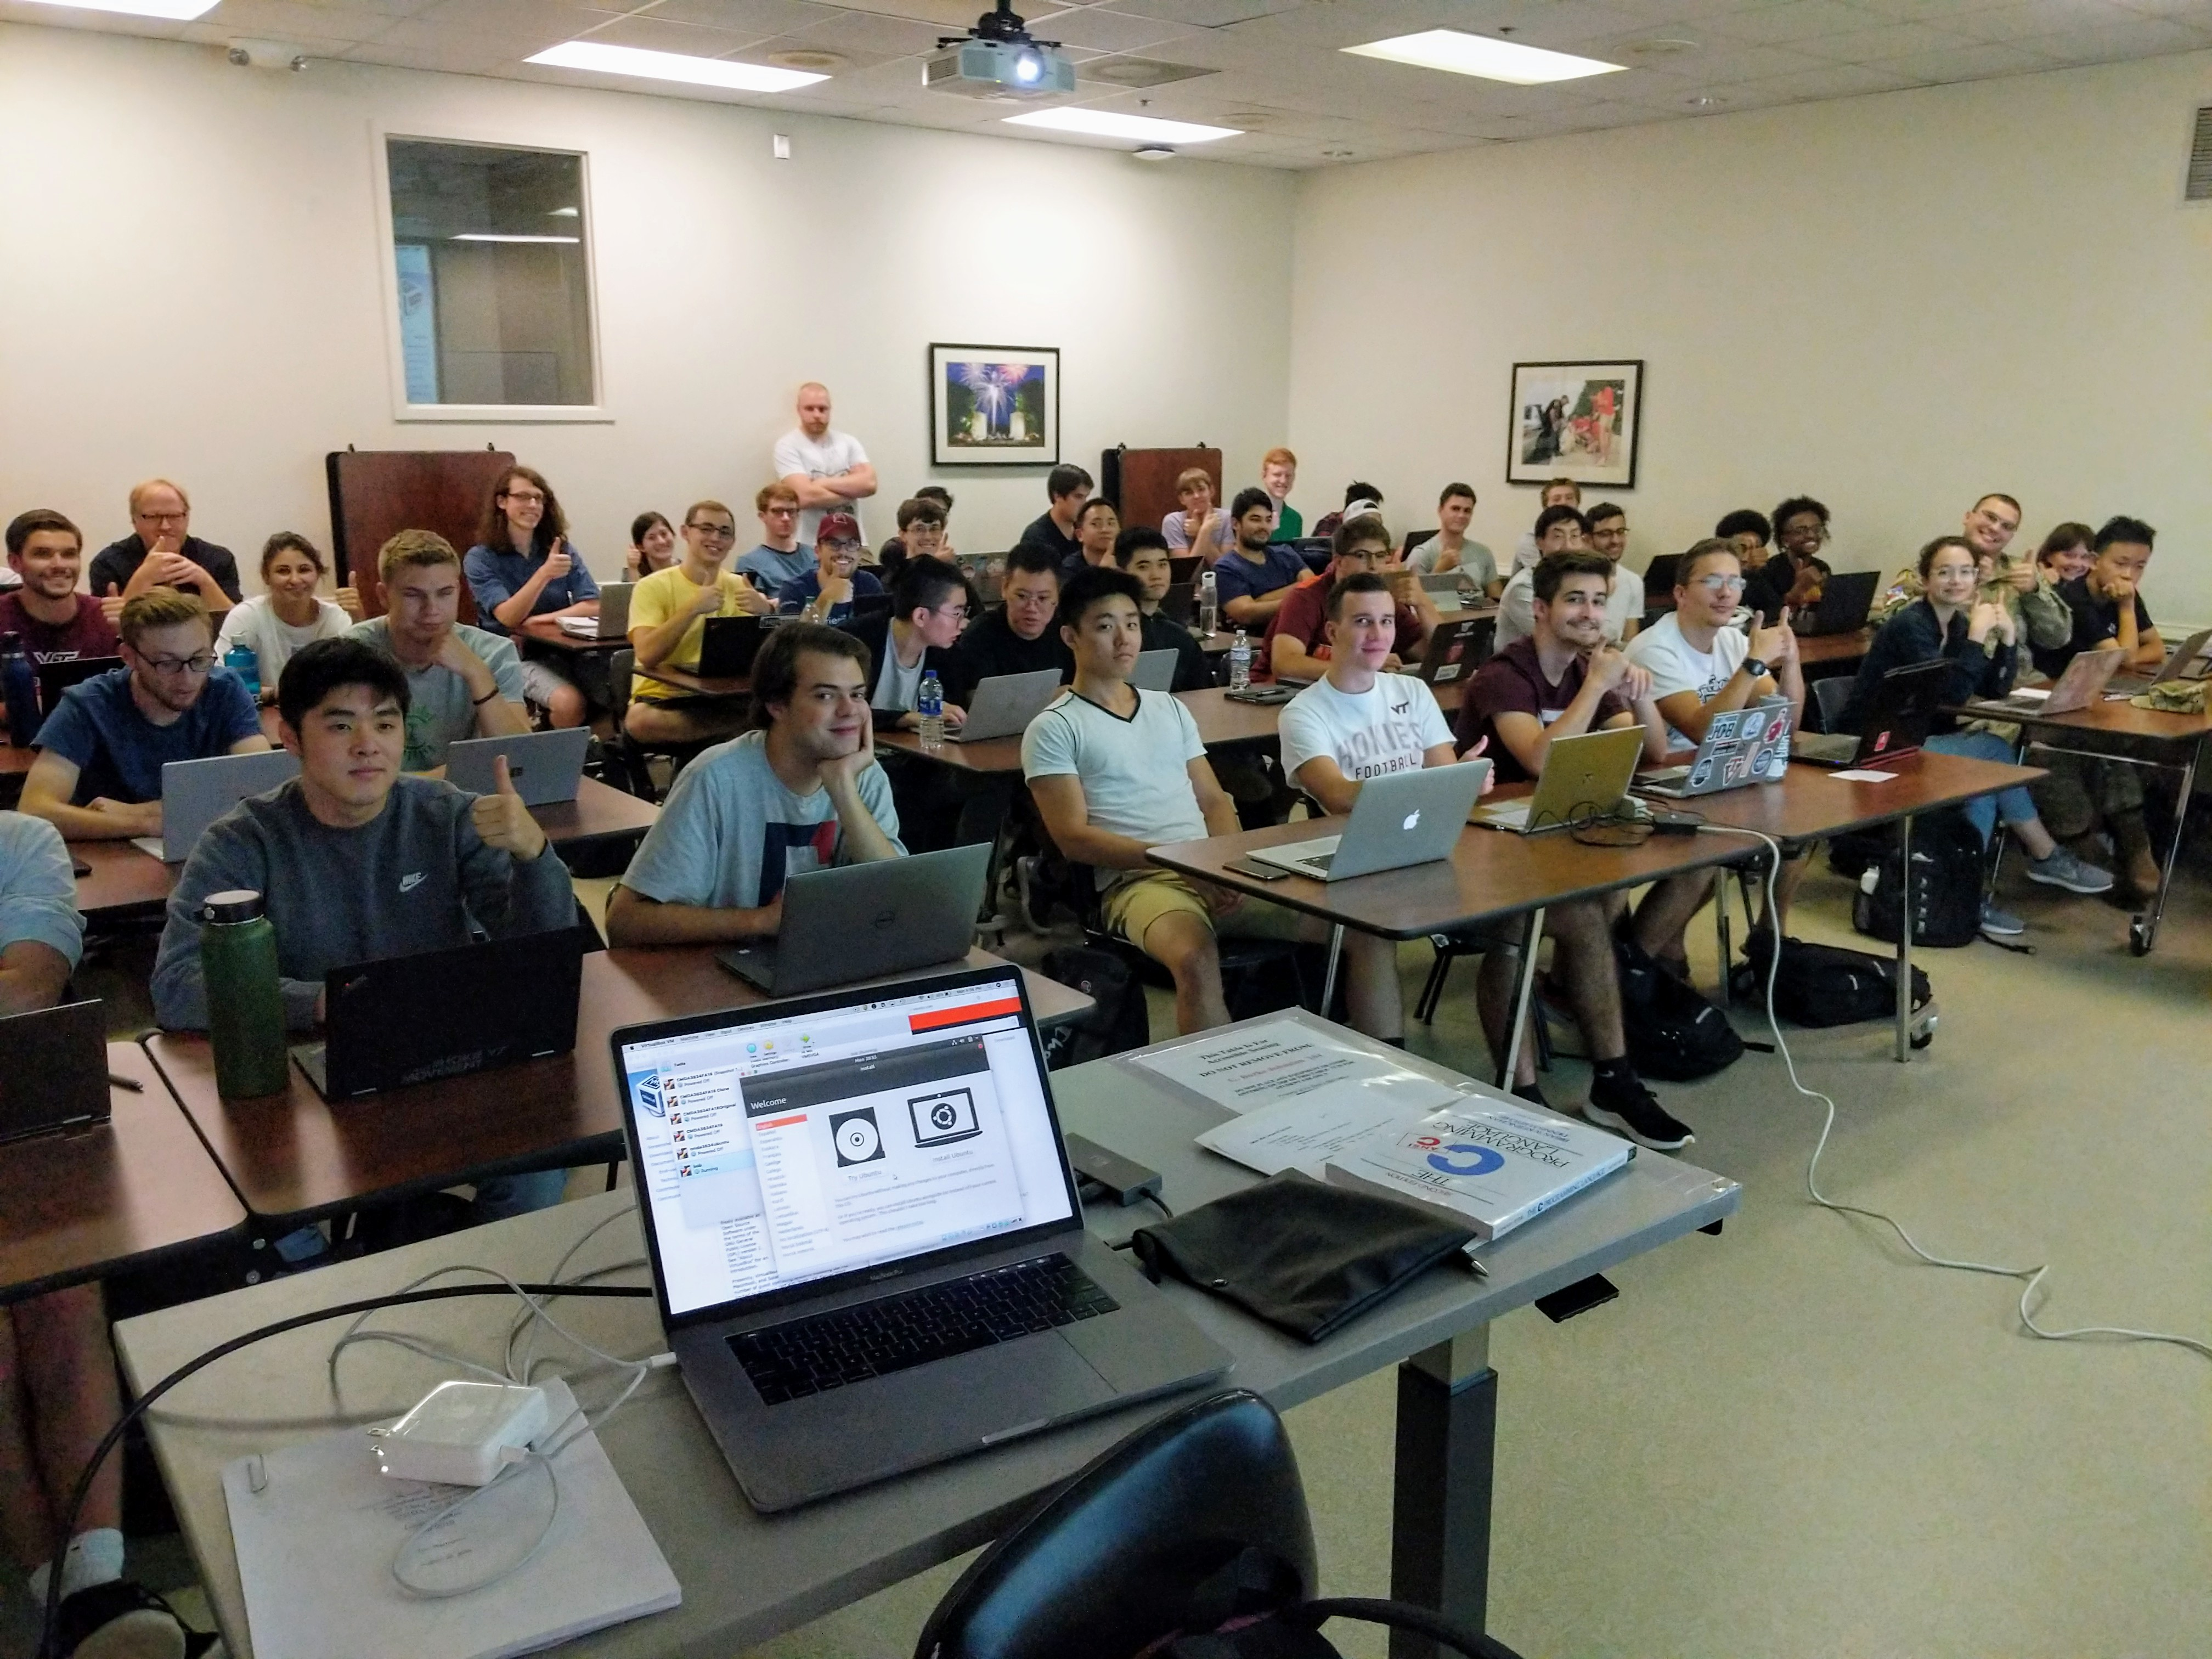
\includegraphics[width=.8\textwidth]{figures/cover/IMG_20190826_165553.jpg}

\begin{minted}{c}
/* PSEUDO-CODE: this code will always deadlock */
int dest   = (rank+1)%size; /* destination = (rank+1) mod size */
int source = (rank-1)%size; /* source      = (rank-1) mod size */

MPI_Recv data info into inBuffer from process source;

MPI_Send data from outBuffer to process dest;
\end{minted}

There is no subtlety here. The above code will always deadlock. In this example all processes are waiting for a message to arrive and no processes are actually sending a message. 

Putting together all these examples we see that relatively simple blocking communications can: serialize message passing, sometimes deadlock if messages are too big, or are guaranteed to deadlock for any message size. This should give you pause given how incredibly similar these codes are and how subtle the differences are that cause communications to succeed or fail. For instance switching the order of \texttt{MPI\_Recv} and \texttt{MPI\_Send} can cause the processes to always fail to communicate. Fortunately we can avoid many of these pitfalls by switching to non-blocking immediate mode point-to-point communications as described in the next section.

\section{MPI: non-blocking point-to-point message passing}

In the last few sections we have seen how brittle MPI communications can be. The brittleness is caused by a few common issues:

\begin{enumerate}
    \item No process is available to post a receive.
    \item MPI does not have sufficient internal buffer space to warehouse messages.
    \item No process can receive data if no process is sending data.
\end{enumerate}

We can mostly avoid all of these issues by switching from using the blocking MPI point-to-point mode of message passing to a non-blocking MPI point-to-point mode. This adds a little code complexity but if done right can avoid many of the potential deadlock traps that blocking mode communications suffer.

To use the non-blocking immediate mode point-to-point send and receive we replace \texttt{MPI\_Send} and \texttt{MPI\_Recv} with \texttt{MPI\_Isend} and \texttt{MPI\_Irecv}. The ``I'' versions return almost immediately as they use the message buffers we supply to them as the actual message buffers. Once they return we do not know whether the message buffer is no longer needed, i.e. we do not know if the message has been successfully sent by \texttt{MPI\_Isend} or received by \texttt{MPI\_Irecv}. We can guarantee that the message buffer supplied to one of these immediate mode functions is safe to use without corrupting the message by calling the blocking \texttt{MPI\_Wait} MPI function. The \texttt{MPI\_Wait} function will block until it is safe to use the buffer.

This three-step process is illustrated in the following where we revisit the example where one process sends a message to a second process.

\begin{minted}{c}
#include <mpi.h>
/* L16/mpiNonBlockingSendRecv.c */
/* two ranks, with rank 0 sending a message to rank 1 */
int main(int argc, char **argv){
 /* initialize MPI library comms  */
 MPI_Init(&argc, &argv);
 
 /* find rank index of current process */
 int rank;
 MPI_Comm_rank(MPI_COMM_WORLD, &rank);

 int N = 10; /* length of message to exchange */
 int n, tag = 999; /* message tag */
   
 if(rank==0){ /* rank 0 sends a message to rank 1 */
   int *outBuffer = (int*) calloc(N, sizeof(int));
   int dest = 1;
   
   for(n=0;n<N;++n) outBuffer[n] = n; 
   
   /* initiate non-blocking send of data to rank 1 */
   MPI_Request outRequest;
   MPI_Isend(outBuffer, N, MPI_INT, dest, tag, MPI_COMM_WORLD, &outRequest);
   
   /* block until send request is completed */
   MPI_Status outStatus;
   MPI_Wait(&outRequest, &outStatus);
 }
 
 if(rank==1){/* rank 1 receives message from rank 0 */
   int *inBuffer = (int*) calloc(N, sizeof(int));
   int source = 0;
   
   /* initiate non-blocking receive of data from rank 0 */
   MPI_Request inRequest;
   MPI_Irecv(inBuffer, N, MPI_INT, source, tag, MPI_COMM_WORLD, &inRequest);
   
   /* block until receive request is completed */
   MPI_Status inStatus;
   MPI_Wait(&inRequest, &inStatus);
 }
 
 MPI_Finalize(); /* shut down MPI library comms */
 return 0;
}
\end{minted} 

In this code we process rank 0 initiates an immediate send (Isend) then waits for it to finish. We did miss an opportunity as we could have added some extra task between the \texttt{MPI\_Isend} and the \texttt{MPI\_Wait} to overlap the communication time with computation. This is sometimes called ``latency hiding'' as it allows us to hide irreducible time of travel for the data with some work and reduce the performance hit for sending a message.

\section{MPI: avoiding deadlock by using non-blocking message passing}

Performance issues aside there is a much more compelling reason to use non-blocking immediate mode point-to-point communications. Recall this pseudo-code is always guaranteed to deadlock (all processes try to receive a message before any process sends data)

\begin{minted}{c}
/* PSEUDO-CODE: this code will always deadlock */
int dest   = (rank+1)%size; /* destination = (rank+1) mod size */
int source = (rank-1)%size; /* source      = (rank-1) mod size */

MPI_Recv data info into inBuffer from process source;

MPI_Send data from outBuffer to process dest;
\end{minted}

The main issue here is that the \texttt{MPI\_Recv} is a blocking call and will not return before the process has received data, and no process is sending data so the code will deadlock. We can resolve this without changing the order of operations by only replacing blocking with non-blocking message passing as follows.

\begin{minted}{c}
/* PSEUDO-CODE: this code will not deadlock */
int dest   = (rank+1)%size; /* destination = (rank+1) mod size */
int source = (rank-1)%size; /* source      = (rank-1) mod size */

MPI_Irecv to initiate receiving data into inBuffer from process source;

MPI_Isend to initiate sending data from outBuffer to process dest;

MPI_Wait for MPI_Irecv request to finish;

MPI_Wait for MPI_Isend request to finish;
\end{minted}

The key part of this is that we delay blocking on the message passing calls until both the \texttt{MPI\_Isend} and the \texttt{MPI\_Irecv} calls are made.
The order in which we issue the  \texttt{MPI\_Isend} and the \texttt{MPI\_Irecv} calls is not important as we are not demanding that they are completed before the functions return. Furthermore, since MPI can access the message buffers even after these functions return the communications will not be impacted by large messages except for the transmission time for large messages being longer. Finally, it is our responsibility to check in with MPI and issue \texttt{MPI\_Wait} calls for every non-blocking message passing operation we requested otherwise we might accidentally corrupt the incoming or outgoing messages by overwriting the contents of the message buffers.

\section{On message latency}

{\bf Definition}: \emph{message latency in message passing refers to the time it takes for a message of zero length to be sent and received.}

The actual measured latency will depend on: network interface controller efficiency, OS software stack, MPI implementation, physical distance the message travels, type of interconnect (wire or fibre), traffic on the network/interconnect, and even in the early days on how the wires were supported.

The latency time associated with passing a message between processes can be critical for performance. The non-blocking MPI point-to-point communications we just introduced are often favored over blocking variants because they offer some potential for ``latency hiding''. That is, while a message is in flight the MPI process can proceed with other calculations instead of just waiting for a message to arrive. However, if the latency is higher (i.e. the flight time for the message is higher than the compute time) then the process will inevitably spin its wheels in the \texttt{MPI\_Wait} while waiting for the message to be sent and/or received. Thus part of the art of writing efficient MPI code is to identify sufficiently large tasks that can be used to achieve latency hiding.

\section{Summary of MPI usage so far}

Table \ref{mpiBasicAPI.tab} summarizes useful MPI functions used above.

\begin{table}[htbp!]
    \centering
    \begin{tabular}{p{1.5in}|p{4in}} \hline
      Action & Action implemented using MPI  functions\\ \hline
       Compile MPI code & \texttt{mpicc -o [EXECUTABLE] [SOURCE FILE NAME].c -lm} \\
       Execute MPI code & \texttt{mpiexec -n [NUMBER OF RANKS] [EXECUTABLE] [ARGS]} \\ \hline \hline
       Initialize MPI &  \texttt{MPI\_Init(\&argc, \&argv);} \\
       Finalize MPI & \texttt{MPI\_Finalize();} \\ \hline
        Get MPI process count &  \texttt{MPI\_Comm\_size([MPI COMMUNICATOR],\&size);} \\
         Get MPI process index (aka rank) &  \texttt{MPI\_Comm\_rank([MPI COMMUNICATOR],\&rank);} \\ \hline
         Blocking send & \texttt{MPI\_Send([SEND BUFFER], [NUM DATA], [MPI DATA TYPE], [DESTINATION], [TAG], [COMMUNICATOR]);} \\
         Blocking receive & \texttt{MPI\_Recv([RECEIVE BUFFER], [NUM DATA], [MPI DATA TYPE], [SOURCE], [TAG], [COMMUNICATOR], [STATUS PTR]);} \\ \hline
         Non-blocking send & \texttt{MPI\_Isend([SEND BUFFER], [NUM DATA], [MPI DATA TYPE], [DESTINATION], [TAG], [COMMUNICATOR], [REQUEST PTR]);} \\
         Non-blocking receive & \texttt{MPI\_Irecv([RECEIVE BUFFER], [NUM DATA], [MPI DATA TYPE], [SOURCE], [TAG], [COMMUNICATOR], [REQUEST PTR]);} \\
         Block until request finishes & \texttt{MPI\_Wait([REQUEST PTR], [STATUS PTR]);} \\
    \hline\end{tabular}
    \caption{Summary of commonly used MPI. Here \texttt{[MPI COMMUNICATOR]} is an MPI Communicator struct, typically \texttt{MPI\_COMM\_WORLD}, i.e. the global communicator for all processes until we start using custom MPI Communicators. Here PTR is short for pointer.}    
    \label{mpiBasicAPI.tab}
\end{table}

% https://www.mpich.org/static/docs/v3.1.x/www3/MPI_Send.html
%https://www.mpich.org/static/docs/v3.1.x/www3/MPI_Recv.html

\section{MPI: tutorials}

\begin{itemize}
    \item Cool MPI tutorial: \href{https://www.codingame.com/playgrounds/349/introduction-to-mpi/introduction-to-distributed-computing}{here}.
\end{itemize}